\documentclass[10pt,a4paper]{article}
\usepackage[utf8]{inputenc}
\usepackage{amsmath}
\usepackage{amsfonts}
\usepackage{amssymb}
\usepackage{amsthm}

\usepackage{float}
\usepackage{subfigure}
\usepackage{framed}
\usepackage{xcolor}

\usepackage{graphicx}
\graphicspath{{images/}}

\definecolor{shadecolor}{gray}{0.9}

\newtheorem{questions}{Question}
\newenvironment{question}
   {\begin{shaded}\begin{questions}}
   {\end{questions}\end{shaded}}

\author{Ram\'on Mart\'inez}
\title{BCPNN and Sequence Learning}

% Paragraph parameters
\setlength{\parskip}{1em}

\begin{document}
\maketitle

\section{Introduction}

\subsection{Sequence Learning}
Section with a brief history of sequence learning in computational nueroscience. Key papers, order, structure. 


The problem started with Lashley \cite{lashley1951problem} Hebb reference. 

The other papers

\subsection{The BCPNN}
Explanation of what is the BCPNN, where does it come from, and some applications. 




\subsection{A simple phenomenological theory of sequence recall}
Successful sequence recall dynamics can be described as three dynamical qualities and their interplay: fixation, erosion and biased transition. 

\textbf{Fixation} is a general mechanism that fixes a state passing a certain point.

Examples of fixation. Attractor dynamics.

\textbf{Erosion} is a mechanisms that eventually suppresses the state after the system has dwell some time on it. 

Examples of erosion 
Spike frequency adaptation \cite{roach2016memory}, feedback inhibition \cite{recanatesi2017memory}. 

\textbf{Biased Transition}, after the state has been eroded the 

Examples of biased transition
Biased by similiarty \cite{recanatesi2017memory}


\section{The BCPNN as a Sequence Learner}
First we can show that the BCPNN can be used do incremental learning \cite{sandberg2002bayesian}. And in particular there is a spike model that can be used to learn sequences \cite{tully2016spike}. 

\subsection{Sequence Learning with only one type of connectivity}
In order to test test the capabilities of the BCPNN neural network as a sequence learning mechanism we will start with a minimal model of it. The idea here is to show the minimal conditions under which the system can successfully reproduce sequential activity and isolate how the parameters and properties of the network interact with each other. After we are equipped with this knowledge we will add more parts to the model and this in turn will provide new capabilities that we will explore later. 

Using the phenomenology presented before, we will explain how the structure of the network in figure \ref{fig:bcpnn_simple_network} and the dynamical equations of the system intertwine to achieve, fixation, erosion and biased transition altogether. 

\begin{figure}[H]
\centering
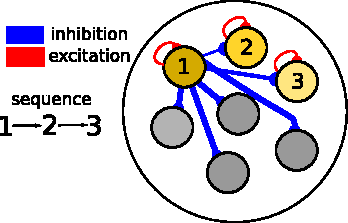
\includegraphics[scale=1.40]{simple_BCPNN.pdf}
\caption{A simple BCPNN network with only one type of connectivity.}
\label{fig:bcpnn_simple_network}
\end{figure}

First the system achieves fixation by the means of the self-excitatory current depicted in red in figure \ref{fig:bcpnn_simple_network}. By itself this mechanism will fix all the patterns at the same time, that is why we need competitive selection.  To solve that problem we will use a winner-takes-all mechanism \cite{yuille1998winner} implemented in the form of equation \ref{eq:simple_bcpnn_max}. This equation ensures that at any point in time only the unit with the higher input current is activated. 


After a particular unit is activated the adaptation current in equations \ref{eq:simple_bcpnn_adaptation} and \ref{eq:simple_bcpnn}  will be the mechanism responsible for the erosion of the pattern. Once a unit is activate for long enough and in the right parameter regime the adaptation current will surpass the self-excitatory current and the pattern will be suppressed. On this light, the time a particular unit remains activated is mostly dependent on the parameters that determine the dynamics of the adaptation and self-excitatory currents and the competitive balance between them. We will make this last relationship quantitative further down in this document. 

Finally, this system would jump randomly among the states if it were not for a proper mechanism of biased transition. For this particular system this is implemented as differential inhibitory weights (illustrated in figure \ref{fig:bcpnn_simple_network} as different widths for the inhibitory connections) that become more and more inhibitory the farther two units are in the sequence. This ensures that once the adaptation currents for a unit becomes big enough the next unit which is the less inhibited one wins the competition and gets prompted to activation by the winner-takes-all mechanism.  

\begin{align}
\tau_m \dfrac{ds_i}{dt} &= g_{beta}\beta_i + g_{w}\sum_{j} w_{ij} o_j + g_a a_i - s_i \label{eq:simple_bcpnn} \\ 
o_i &=  \delta_{i, argmax(s)} \label{eq:simple_bcpnn_max} \\ 
\dfrac{da_i}{dt} &= o_i - a_i \label{eq:simple_bcpnn_adaptation}
\end{align}

In order to illustrate the described phenomena of how the dynamics of the system work together we show an example of a successful sequence recall in figure \ref{fig:bcpnn_simple_recall}. In the recall process we cue the first unit of the sequence by clamping it by a short period of time ($\sim 100ms$). We then let the system evolve on its own and given the right combination of parameters a sequence is effectively recalled if all the units are activated in the expected order. 

It is important to note that in this case we utilized a tailor-made connectivity matrix to clarify the relationship between the different component of the dynamics. Further down we will show how the same effect can be effectively achieved with a matrix that emerges from a self-organized learning process.  

\begin{figure}[H]
\centering
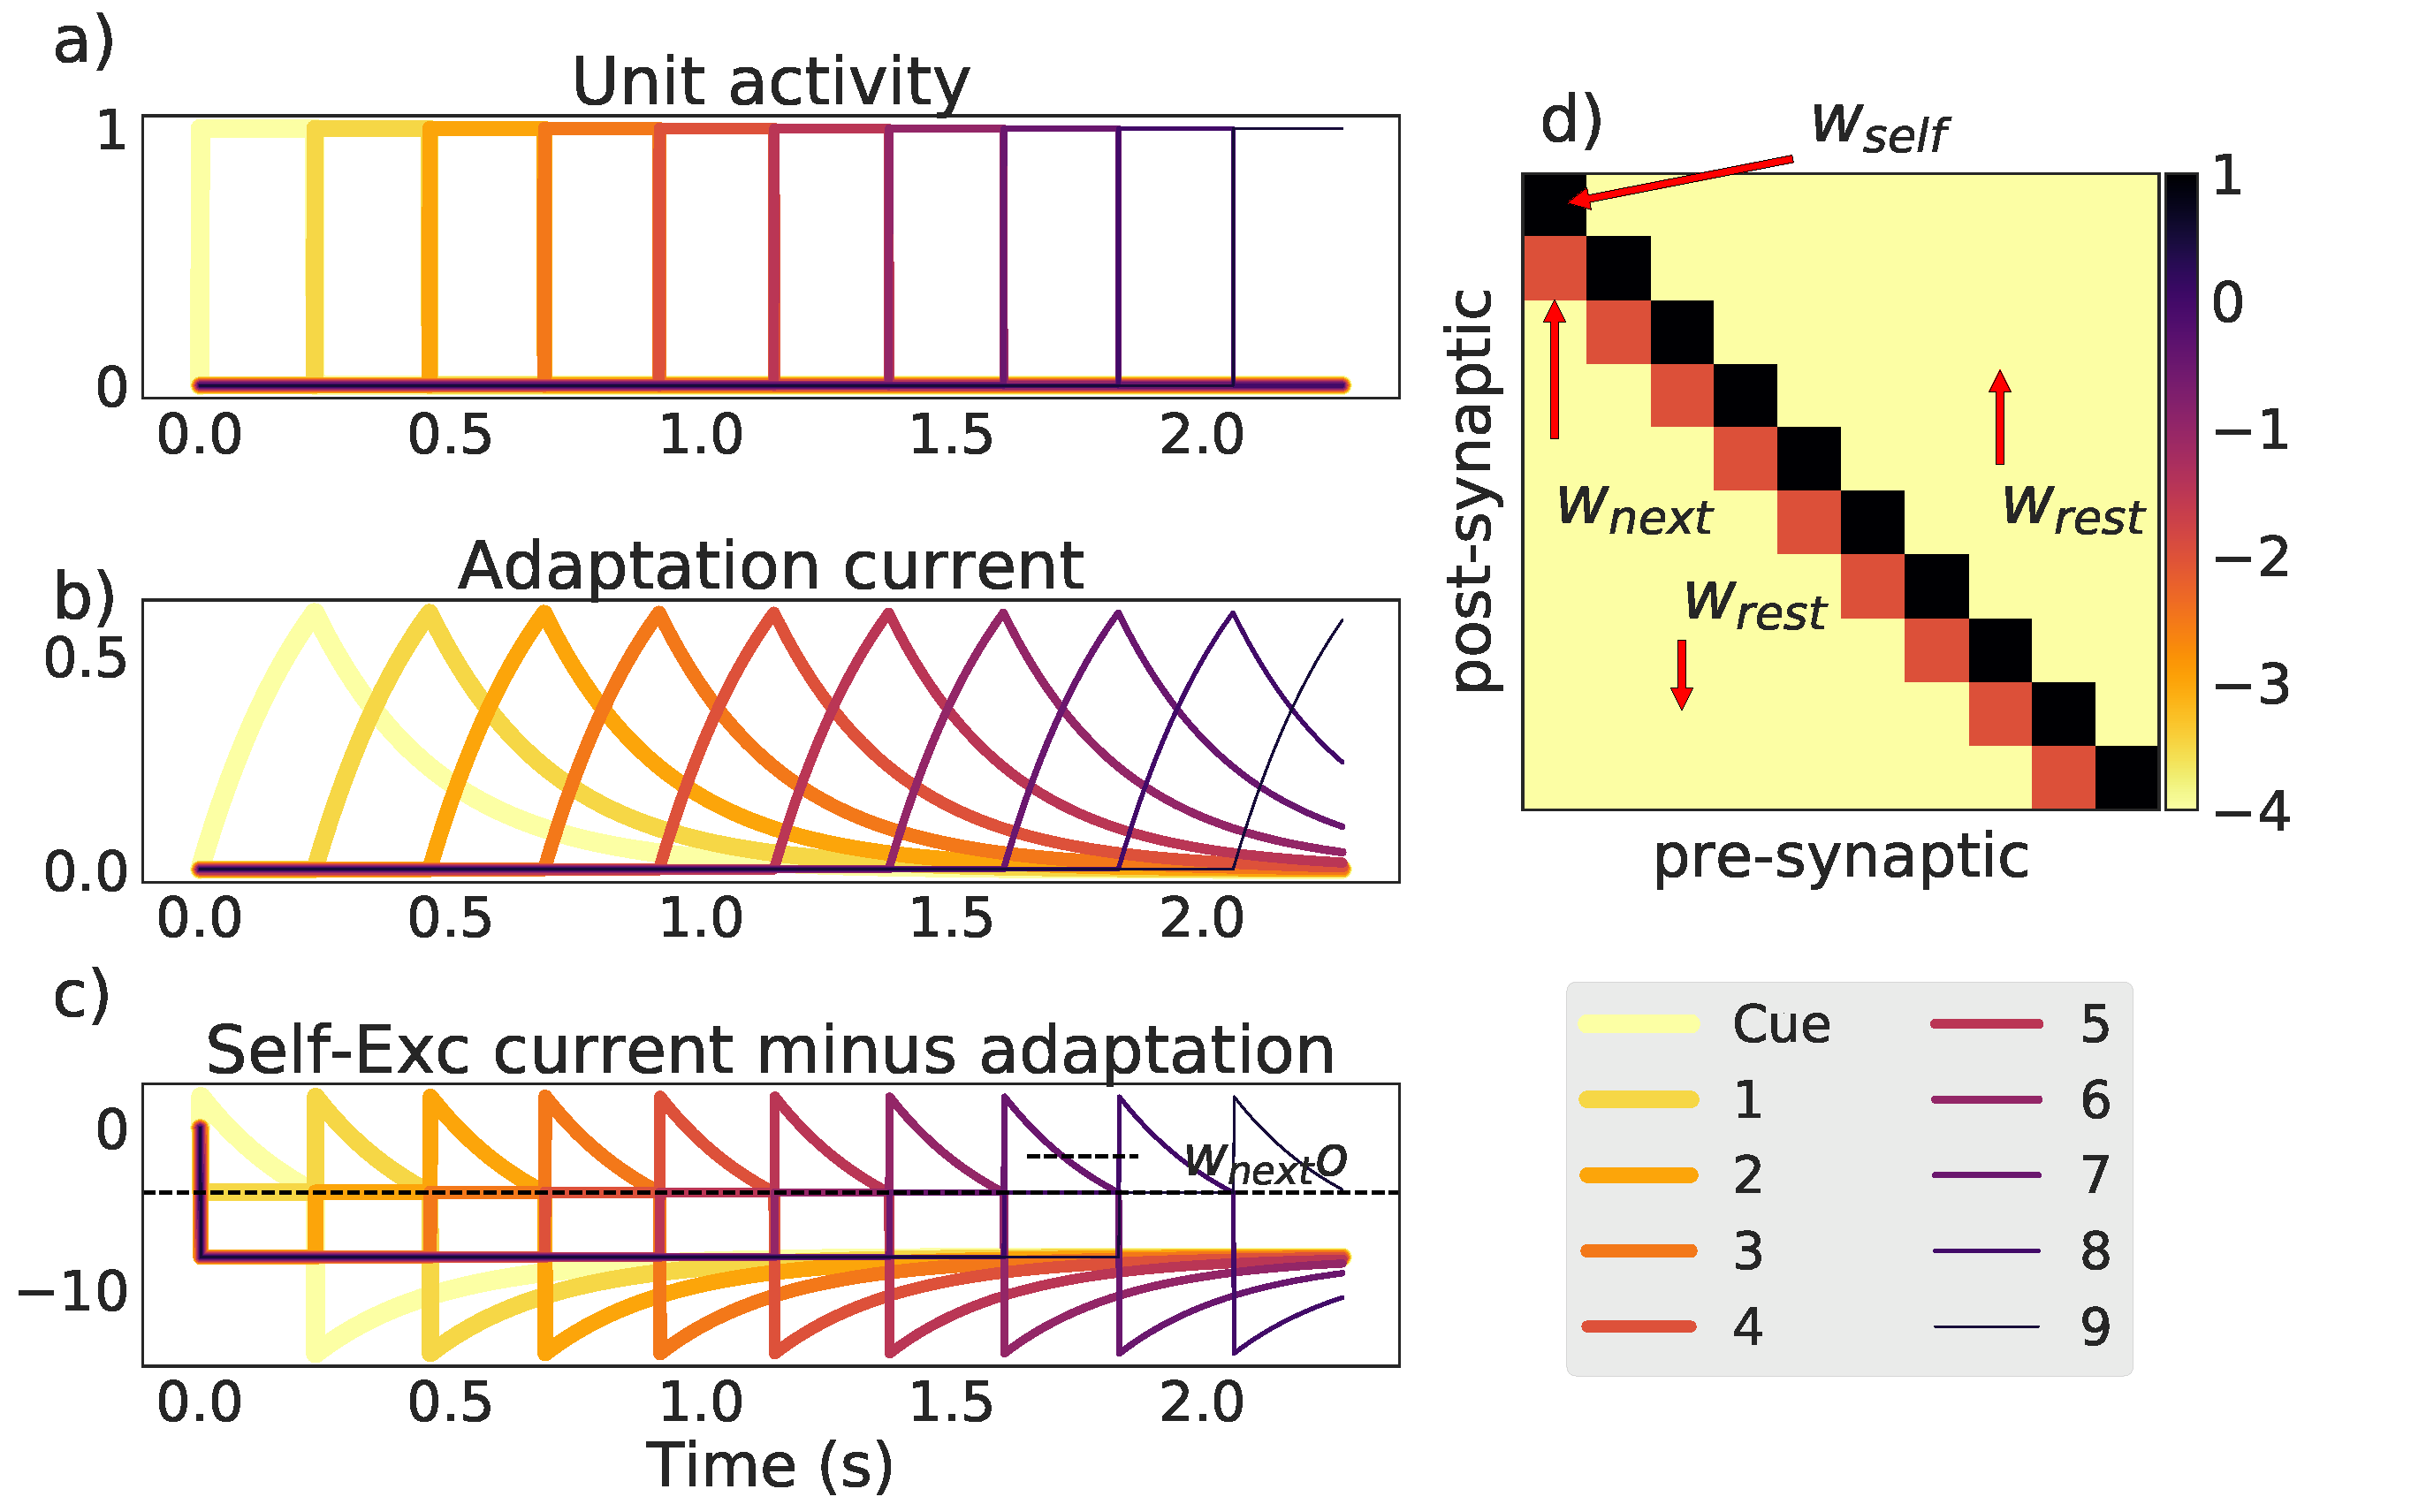
\includegraphics[scale=0.26]{simple_bcpnn_recall.pdf}
\caption{An instance of recall in the simple BCPNN neural network. a) Unit activity starting with the cue. b) the time course of the adaptation for each unit. c) the self-excitatory current minus the adaptation current, note that this quantity crossing the value of $w_{next}$ (depicted here with a jagged line) marks the transition point from one unit to the next. d) The connectivity matrix where we have included pointers to the three most important quantities $w_{self}$ for the self-excitatory weight, $w_{next}$ for the inhibitory connection to the next element and $w_{rest}$ for the rest of the connections.}
\label{fig:bcpnn_simple_recall}
\end{figure}

We will now proceed to characterise the properties of the simplified version of the BCPNN. We will do this in two steps, first we will explain the recall properties of the system. This is mainly an answer to the question of which parameters of the network guarantee successful recall. Given the simplicity of the system it turns out that this can be done simultaneously with the characterization of the persistence time, this is, the length of time that a particular unit becomes activated.  Second, we will characterize the learning learning properties of the system, that is, if we subject the system to different presentations of the sequence under the BCPNN plasticity rule, in which conditions the weights learneed are such that the systme recall succesfull?

\subsubsection{Recall properties}
If we have system with only one type of connectivity, and perfect soft-max selectivity one state will be suppressed in favor of the other as soon as the support of the second state is bigger. In more detail, if we start with a system where the first unit is activated its own support will be $s_1 = g w_{self} - a(t)$ where a is the adaptation time. Where the adaptation current is increasing in time for as long as the first unit is activated. On the other hand the second unit is receiving a constant current to its support $s_2 = g w_{next}$, if this process continues by continuity there will be a point when:

\begin{align*}
s_1 &= s_2 \\
gw_{self} - g_{a} (1 - e^{\frac{t}{\tau_a}}) &=  g w_{next}
\end{align*}


Where we have substituted the proper term for adaptation. We can solve the equation equation above to obtain the persistence time:

\begin{align}
T_{persistence} = \tau_{a} \ln \left(\frac{g_a}{g_a - g_w (w_{self}  - w_{next})} \right) \label{eq:simple_bcpnn_persistence_time}
\end{align}

We show comparisons between this theory and simulations in equation \ref{fig:simple_bcpnn_comparison} we will now elaborate why the curves look the way they do.

\textbf{Adaptation current time constant} $\mathbf{\tau_{a}}$ \\
We explain here how the persistence time dynamics depend on $\tau_a$ the time constant of the adaptation current. A priori, the longer the adaptation time constant the longer it will take to the adaptation time current to erode the pattern. From equation \ref{eq:simple_bcpnn_persistence_time} we can observe that the relationship is linear which is exactly what we get in figure \ref{fig:simple_bcpnn_comparison} a).  

\textbf{Adaptation current gain $g_a$}
The adaptation time current is actually a limiting factor in the succesfull recall of a sequence. If the adaptation current is not big enough that it can overcome the difference between the self-excitatory current and the inhibitory current of the next element then the system will get stuck forever in the same state, in other words, the system of erosion will not work. Therefore we need the value to be bigger the difference in weights multiplied by the gains. Once we have overcome this threshold the behavior becomes obvious, the bigger the gain of the adaptation current the faster this current will overcome the self-excitatory one and therefore the persistence time will be bigger. We illustrate this behavior in figure \ref{fig:simple_bcpnn_comparison}. An important point regarding the behavior of the persistence is to be noted here, it presents a singularity. From equation \ref{eq:simple_bcpnn_persistence_time} denominator we can see that the expression will diverge when $g_a = g_w (w_{self} - w_{next})$ and we can see that behavior reflected accurately in the graph. This divergences are important because 

\begin{figure}[H]%
    \centering
    \subfigure[$\tau_a$]{{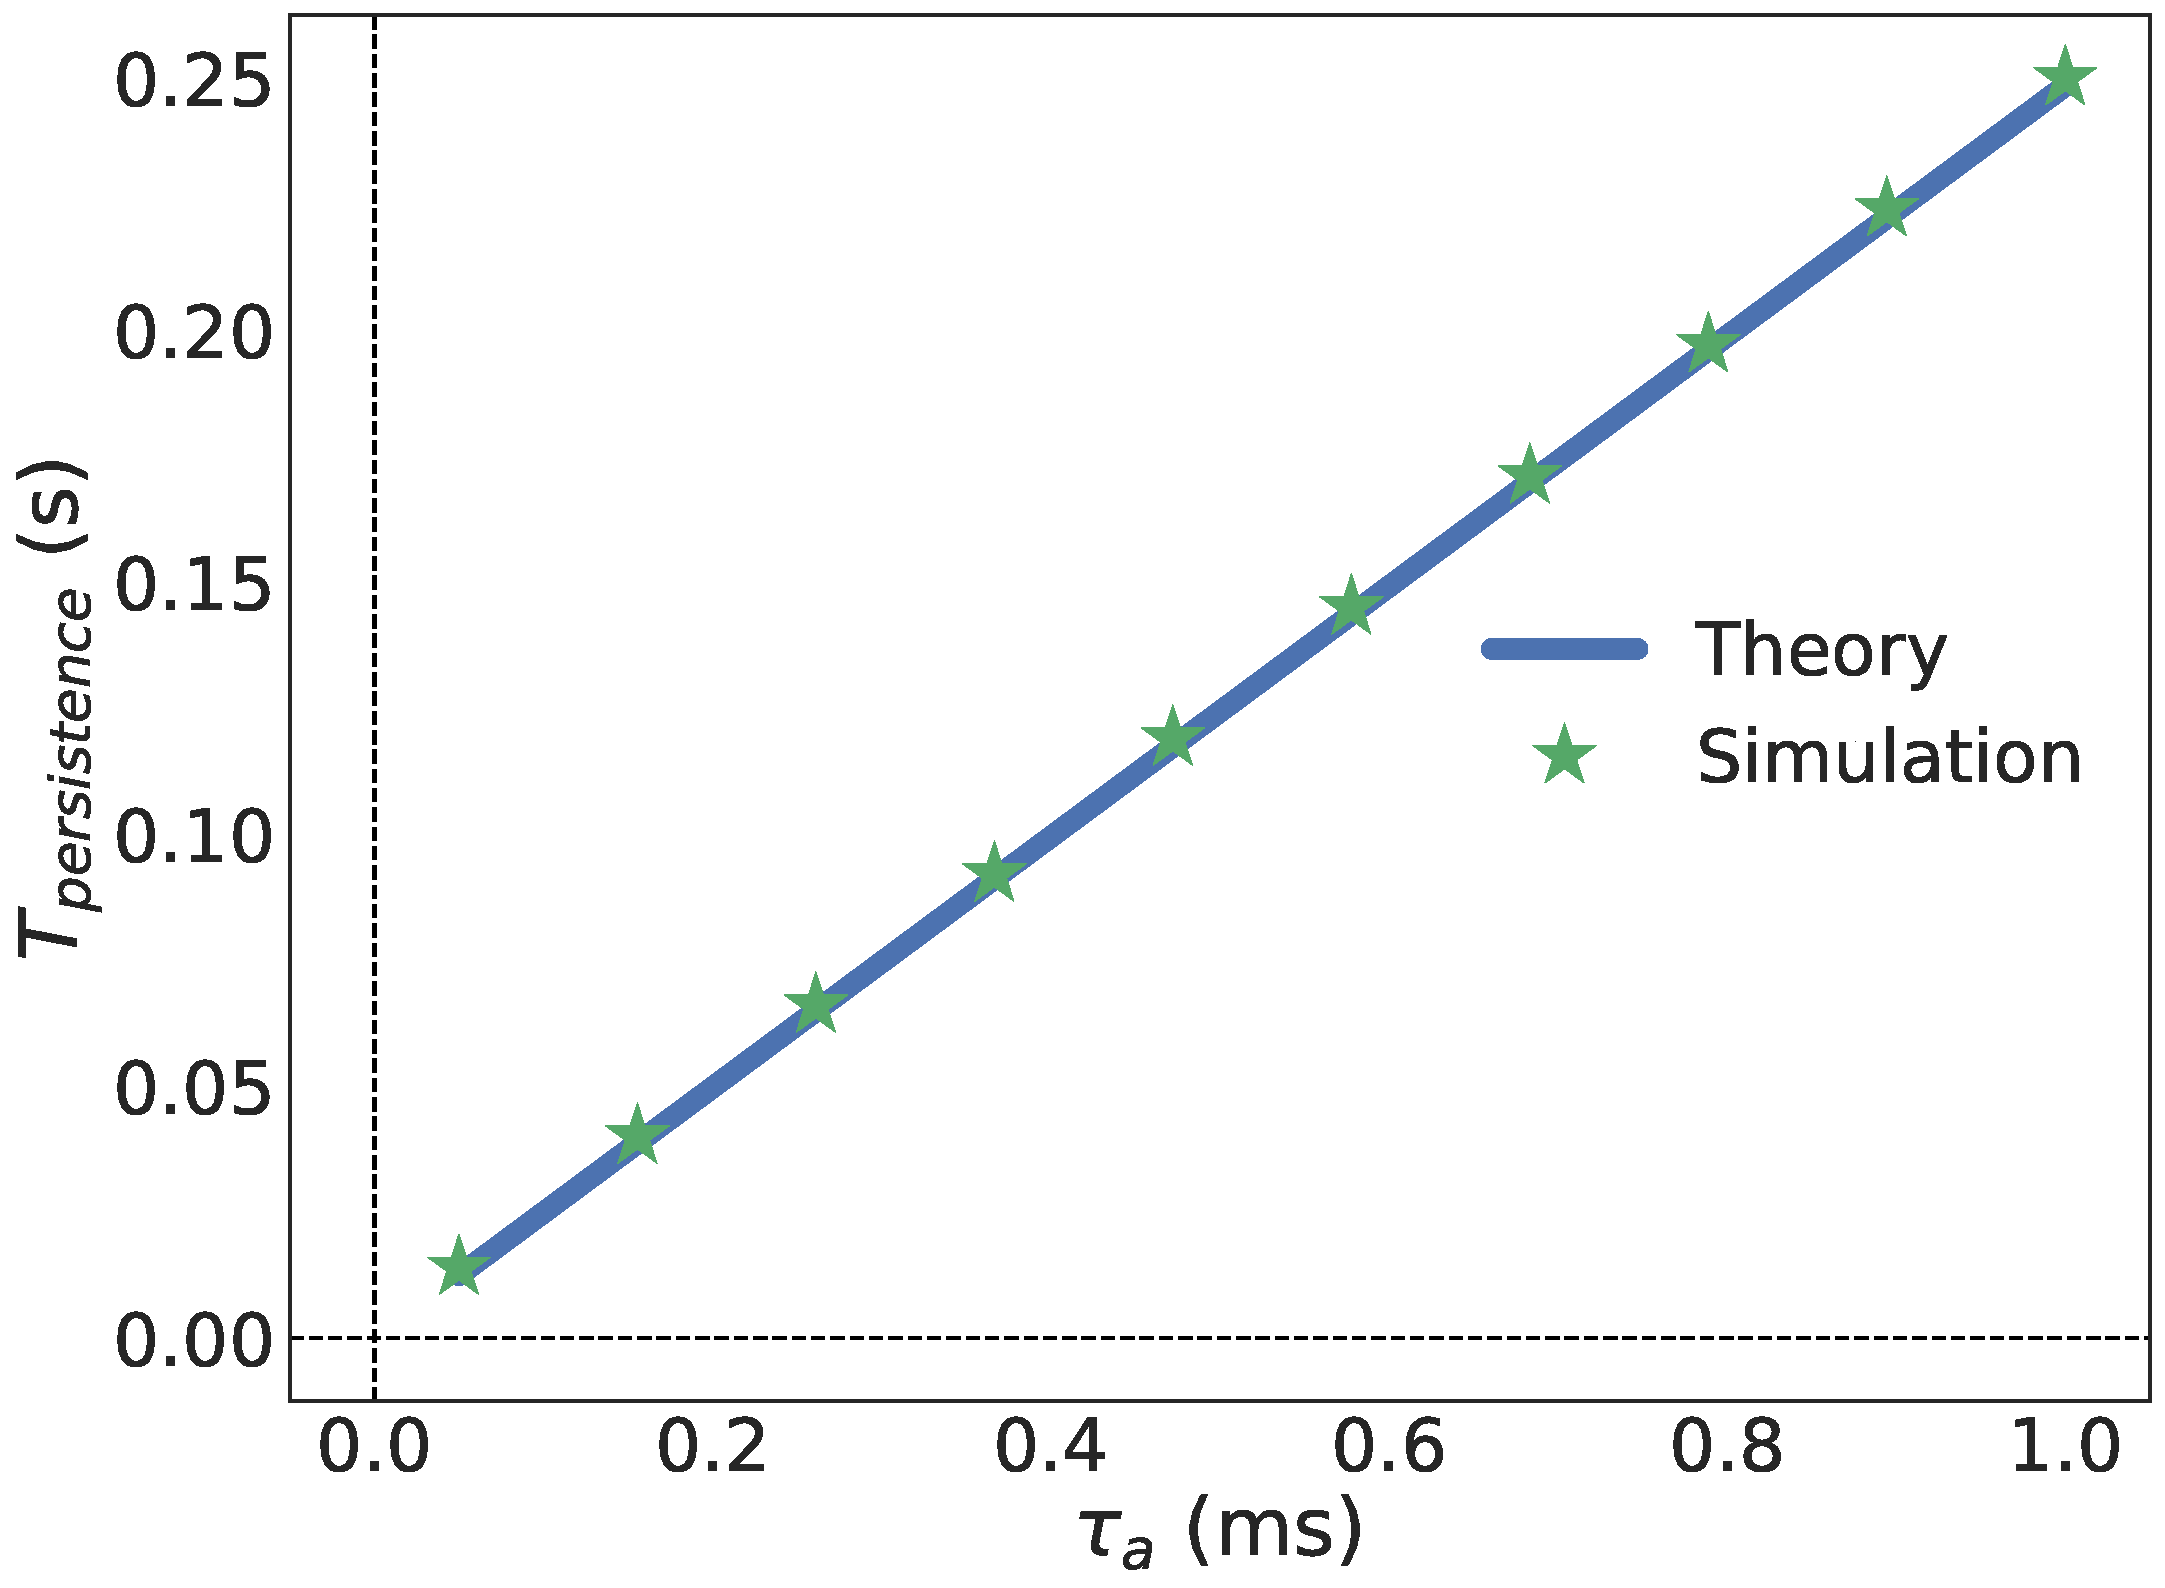
\includegraphics[width=5cm]{simple_bcpnn_tau_a.pdf} }}%
    \qquad
    \subfigure[$g_a$]{{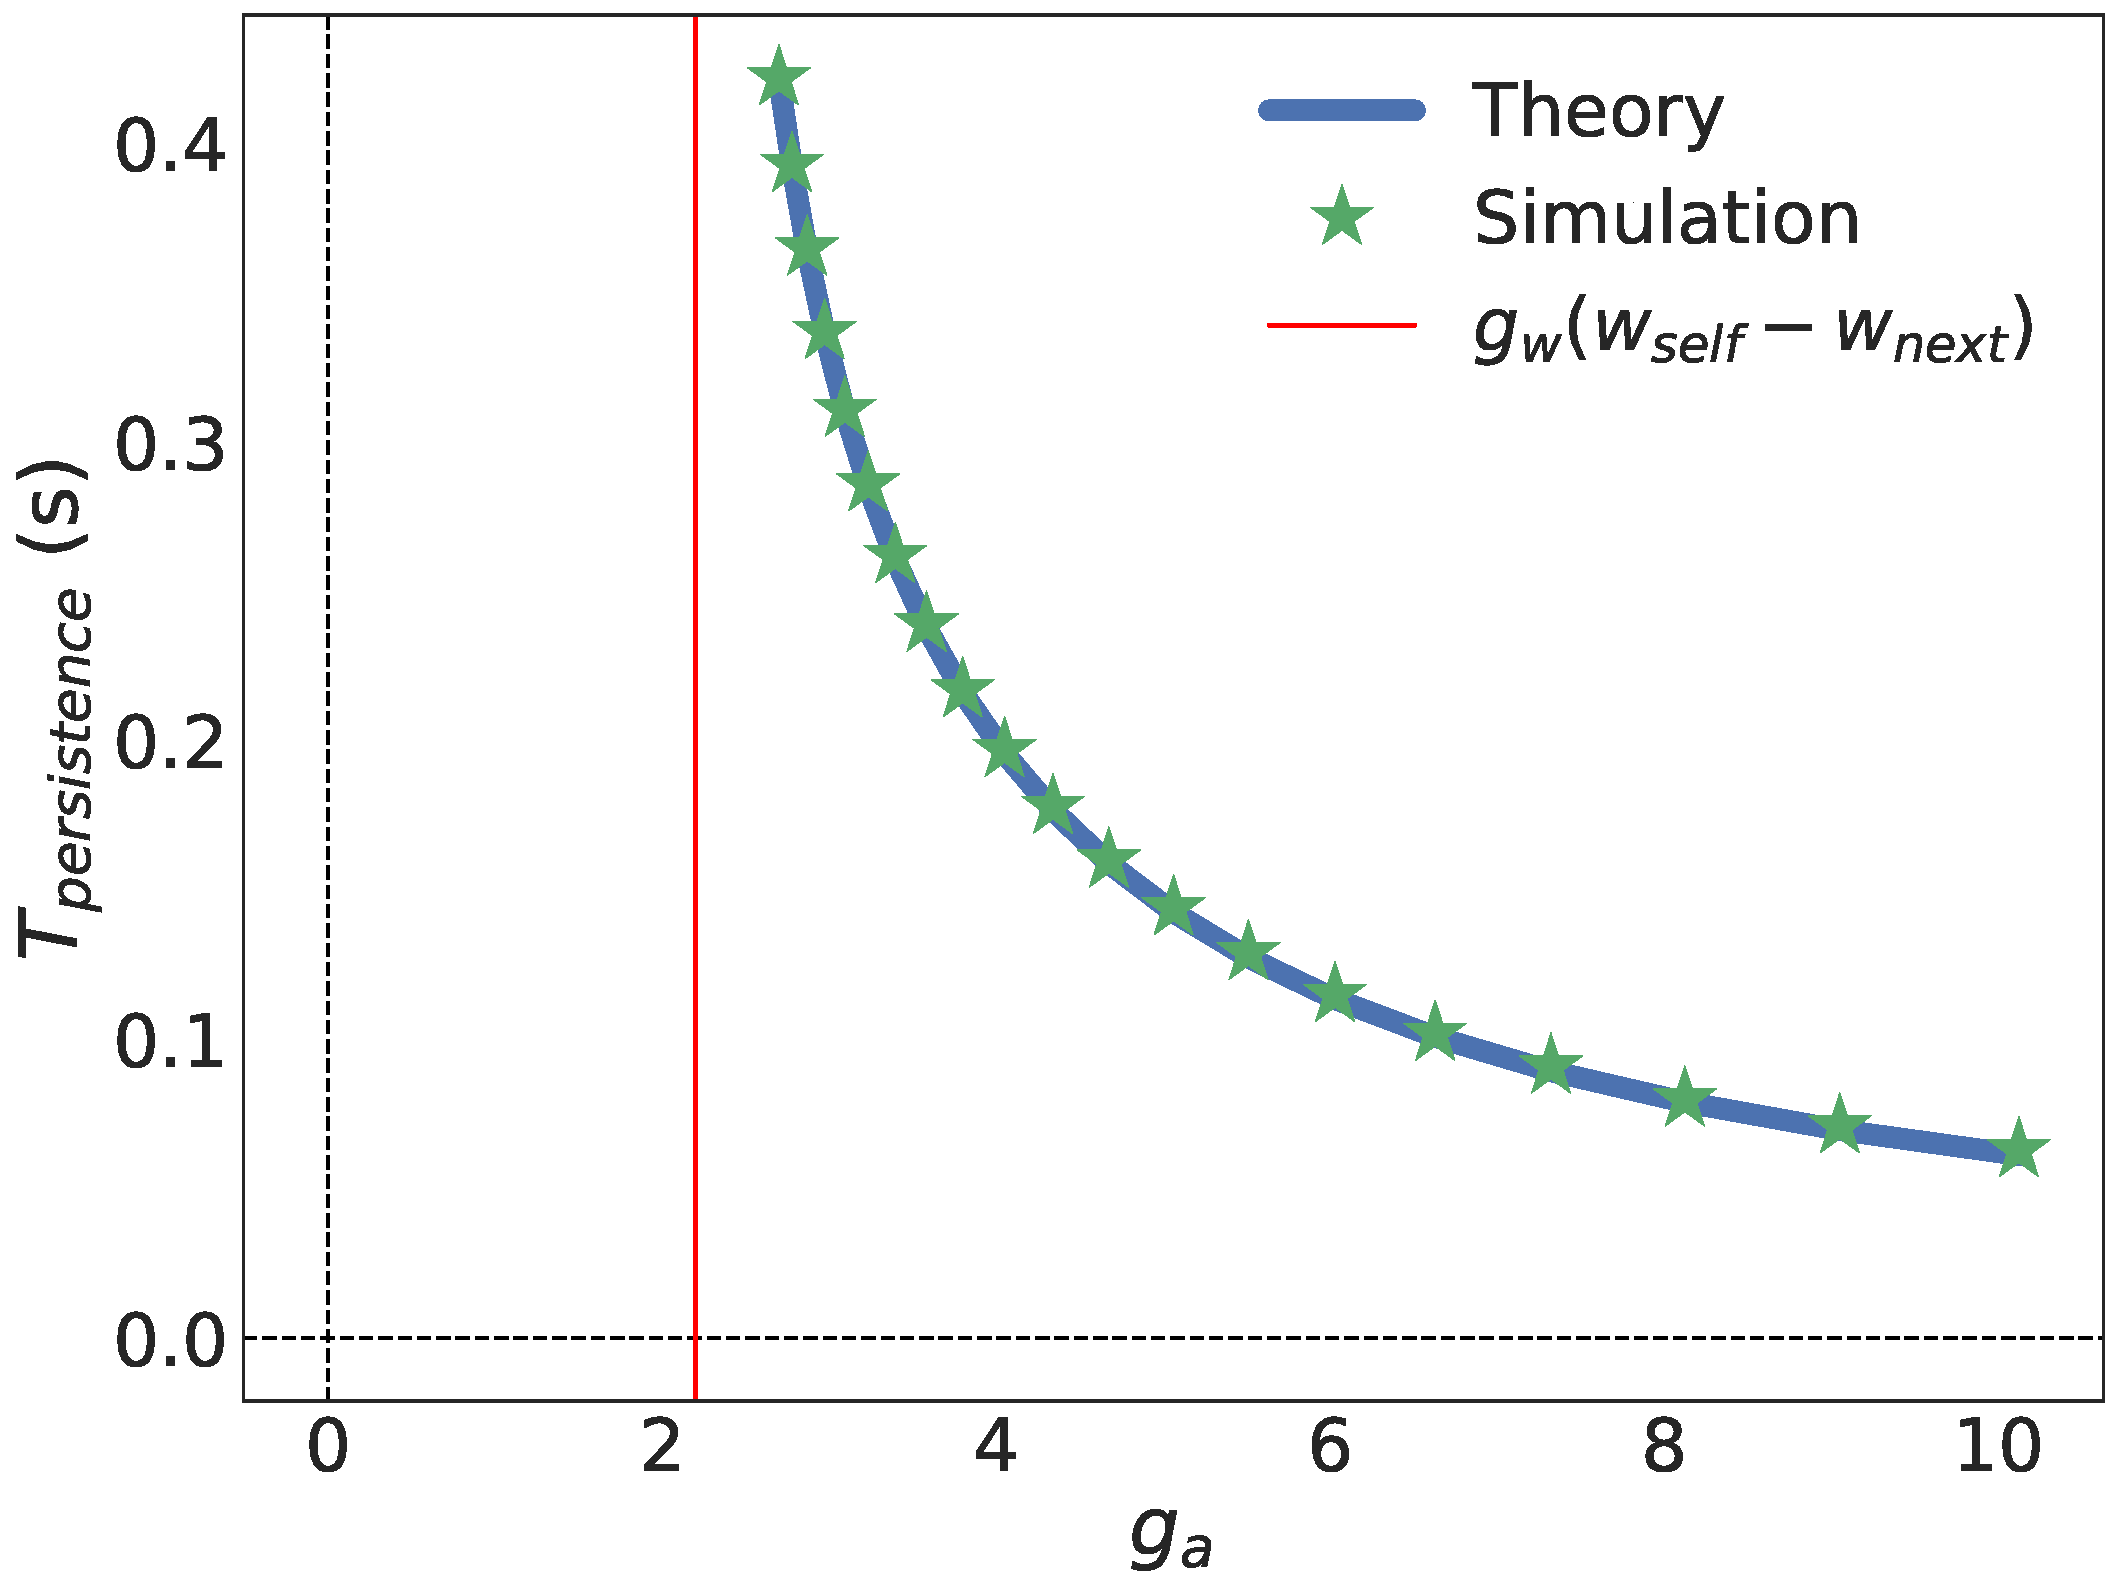
\includegraphics[width=5cm]{simple_bcpnn_g_a.pdf} }}%
    \hfill
    \subfigure[$g_w$]{{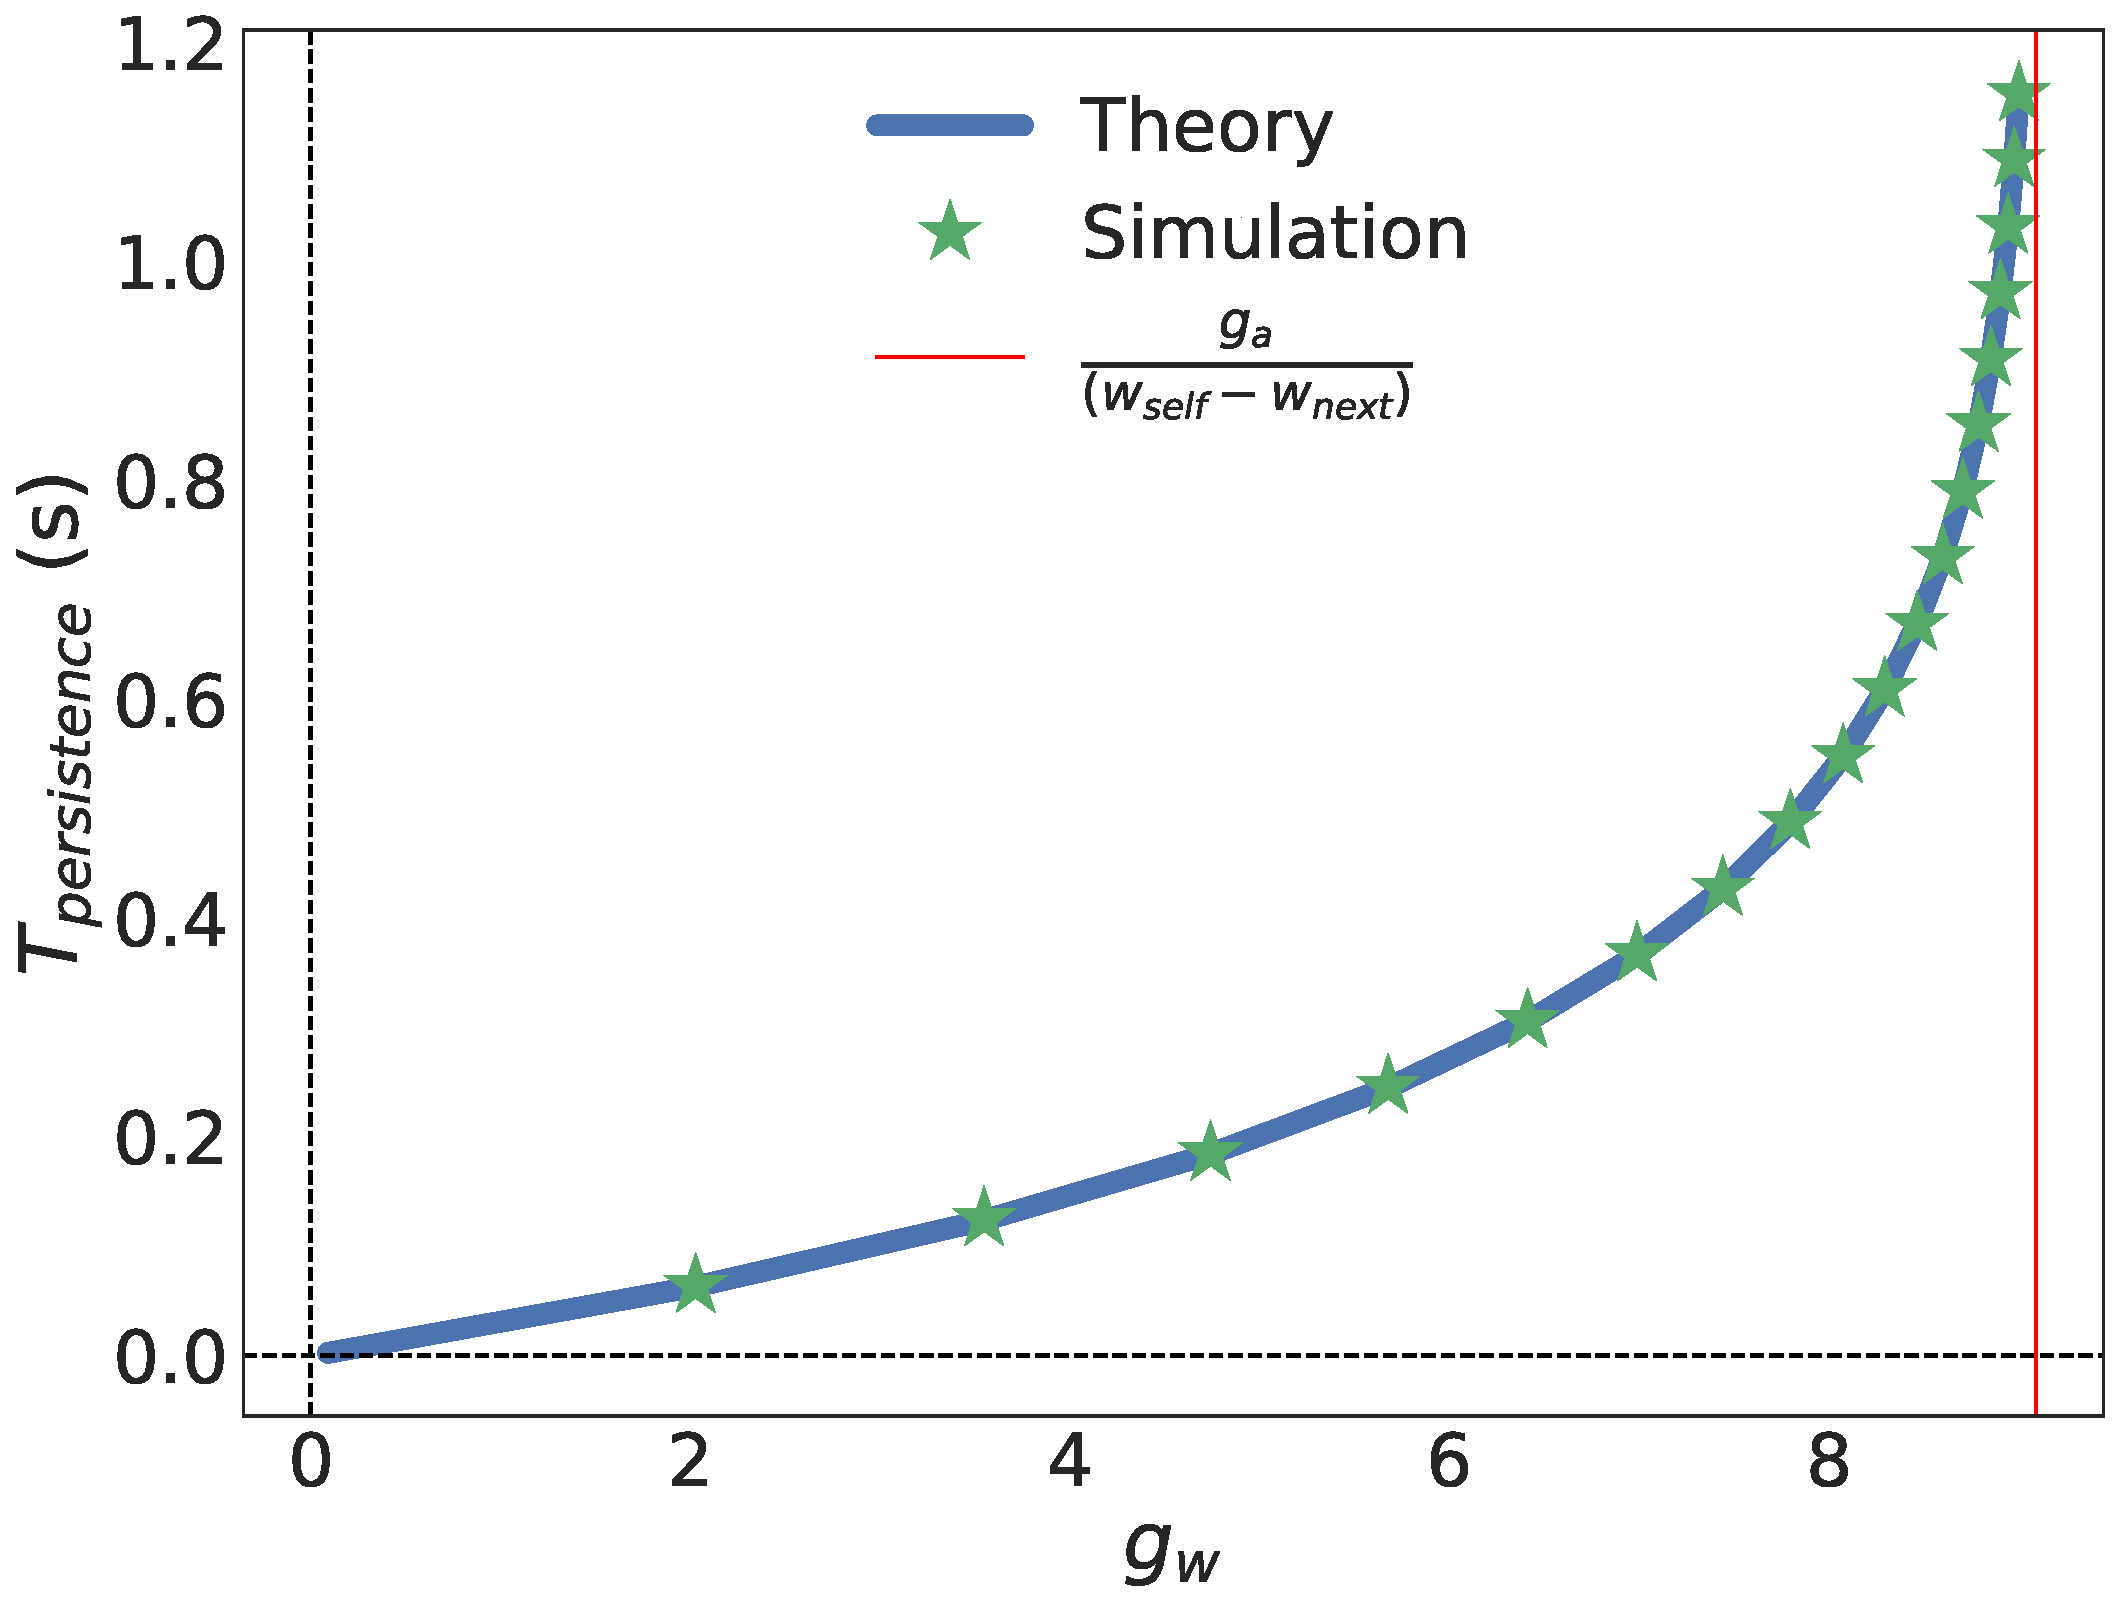
\includegraphics[width=5cm]{simple_bcpnn_g_w.pdf} }}%
     \qquad
    \subfigure[$w_{next}$]{{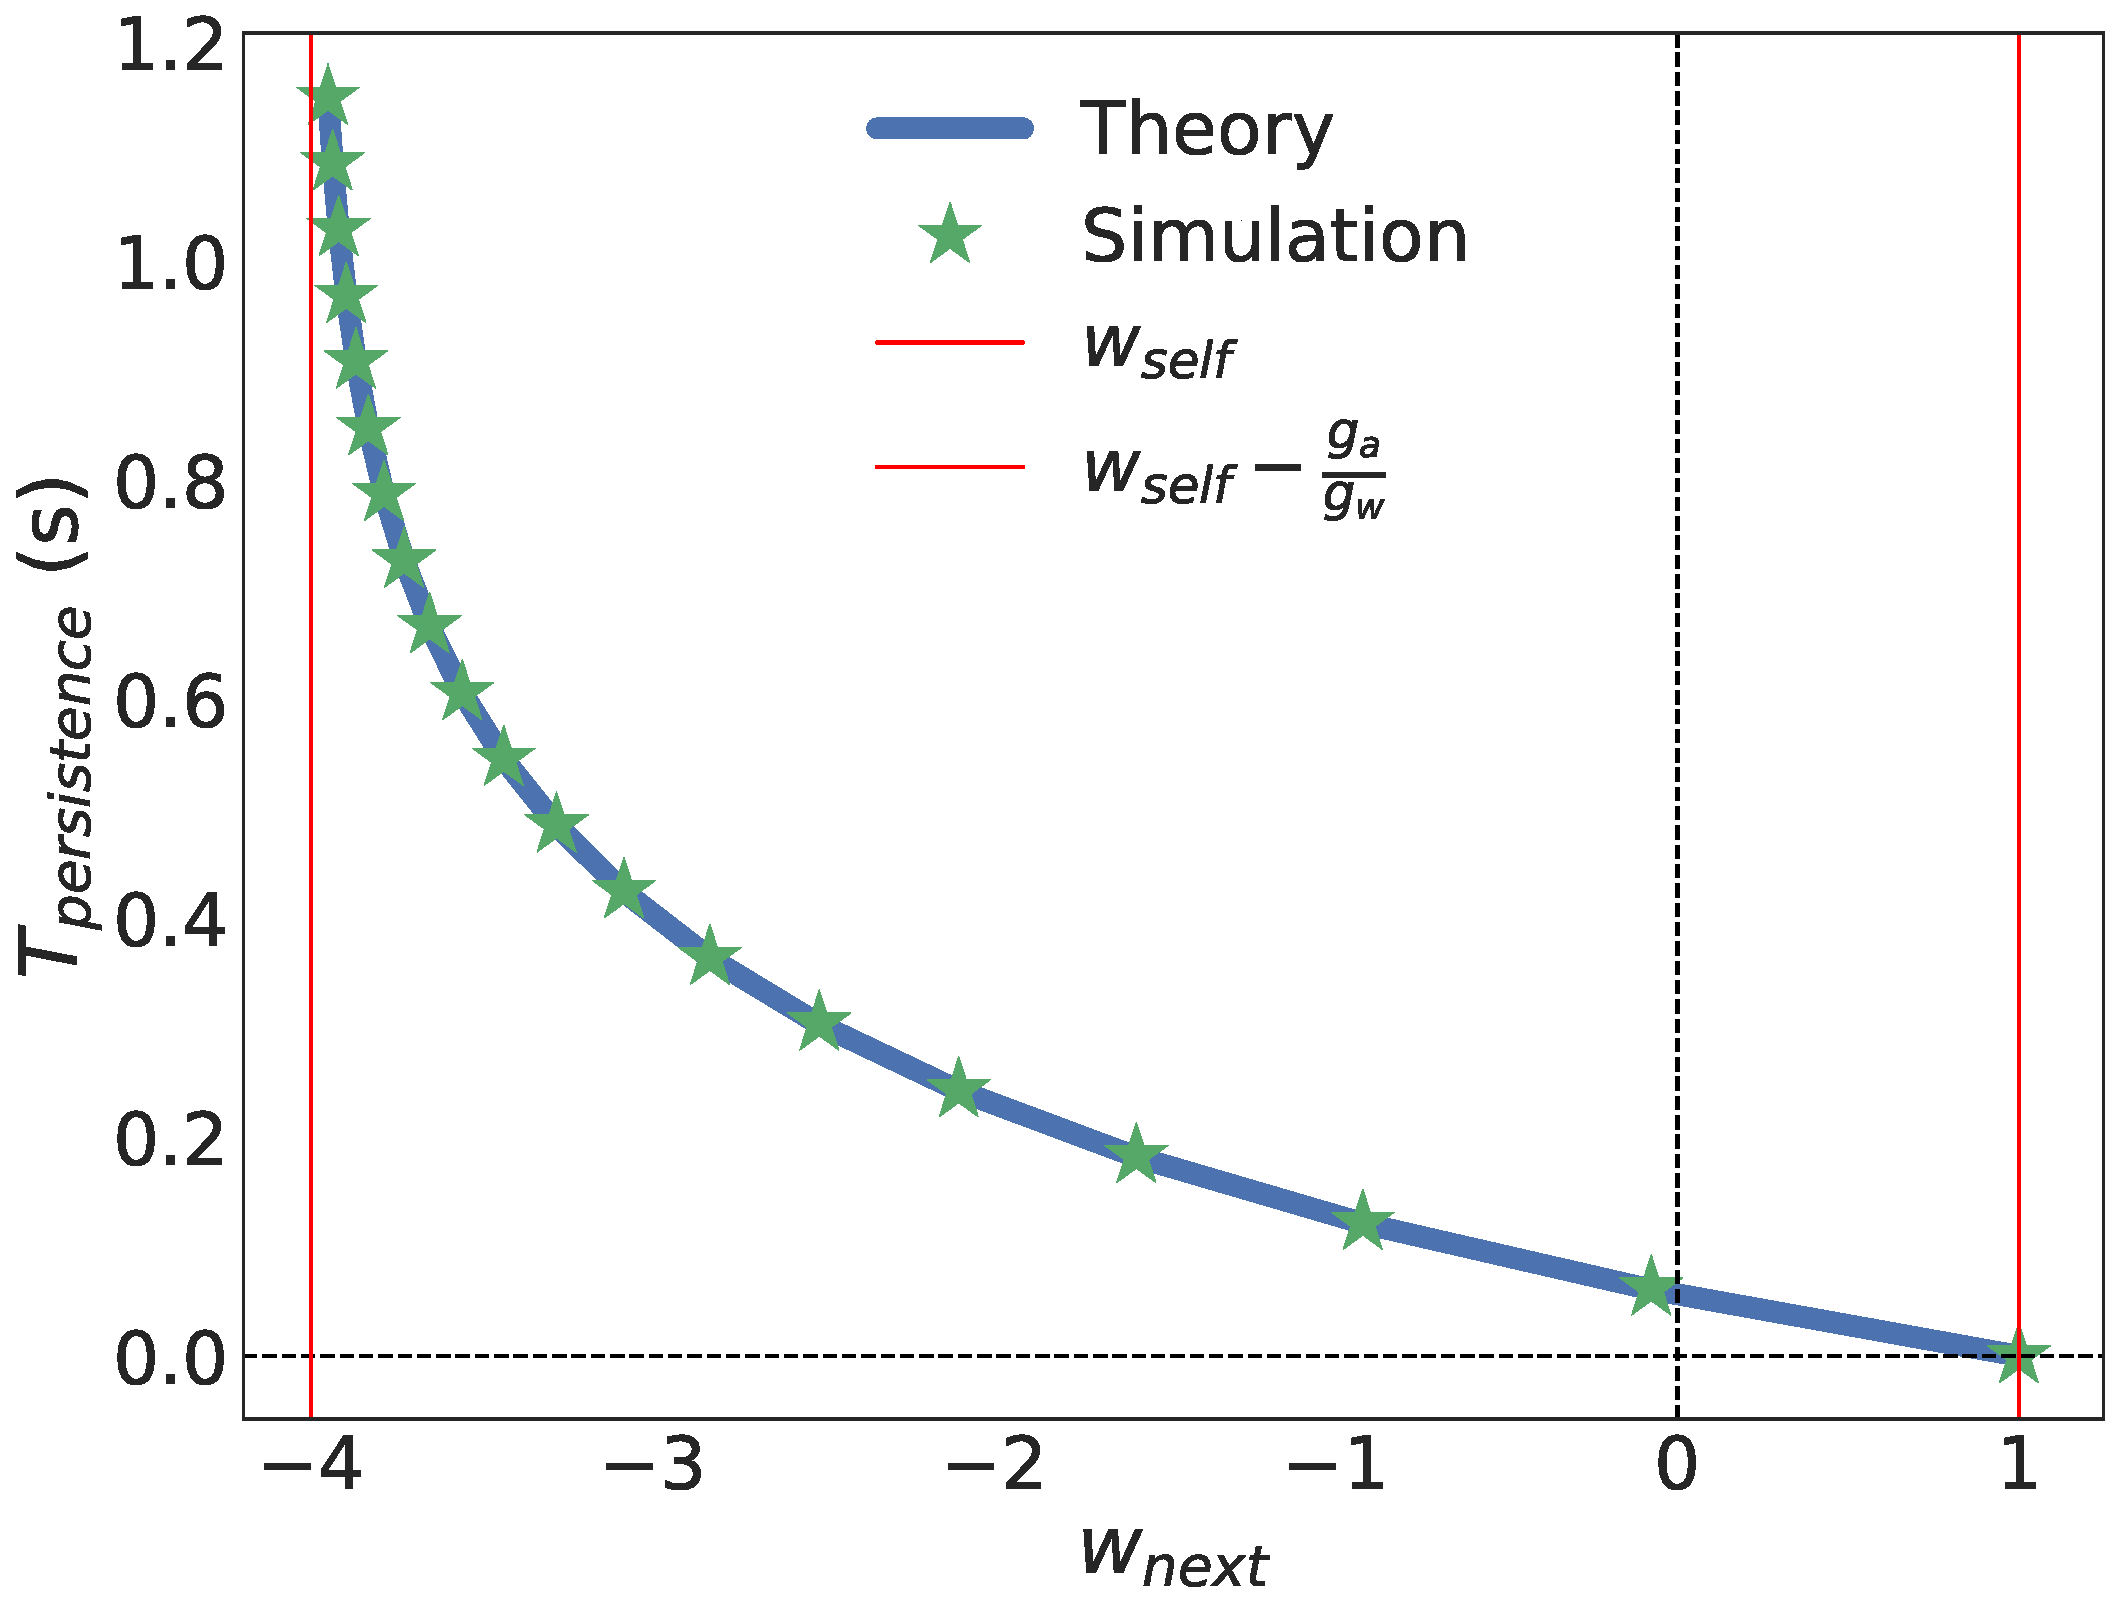
\includegraphics[width=5cm]{simple_bcpnn_w_next.pdf} }}%
    \caption{Persistence time relationship with the parameters. a) We can appreciate that the persistence time grows linearly with $\tau_a$, the adaptation current time constant. b)   }
    \label{fig:simple_bcpnn_comparison}%
\end{figure}

\textbf{Weight Gain}


\textbf{Next weight value}

\subsubsection{Learning Properties}
Once we know the dynamics of the system given a certain matrix the natural question to consider is whether we can learn the weight matrix. As described in \cite{sandberg2002bayesian} with the help of traces we can add on-line learning capabilities to the BCPNN neural network. 

\begin{align}
\tau_z \dfrac{dz_i}{dt} &= o_i - z_i \\
\tau_p \dfrac{dp_i}{dt} &= z_i - p_i  \\  
\tau_p \dfrac{dp_{ij}}{dt} &= z_i z_j - p_{ij}\\
w_{ij} &= \log(\frac{p_{ij}}{p_i p_j}) \\
\beta_i &= \log(p_i) 
\end{align}

\textbf{An example of learning}
Here put a picture of how learning looks like under this scheme.

\textbf{The training protocol}
Here we describe the training protocol. The first to note is that we train the neural network by clamping a given set of units in the order of a given sequence for a given time. More specifically a training protocol is characterized by the following quantities. First there is the \textbf{training time} for a given element of the sequence, that is, the time that element remains activated. 

\begin{figure}[H]
\centering
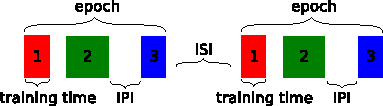
\includegraphics[scale=1.40]{protocol.pdf}
\caption{The training protocol. IPI stands for inter pulse interval and ISI for inter sequence interval. Explanations in the text.}
\label{fig:bcpnn_simple_network}
\end{figure}




\textbf{Training Time}


\begin{figure}[H]%
    \centering
    \subfigure[$\tau_a$]{{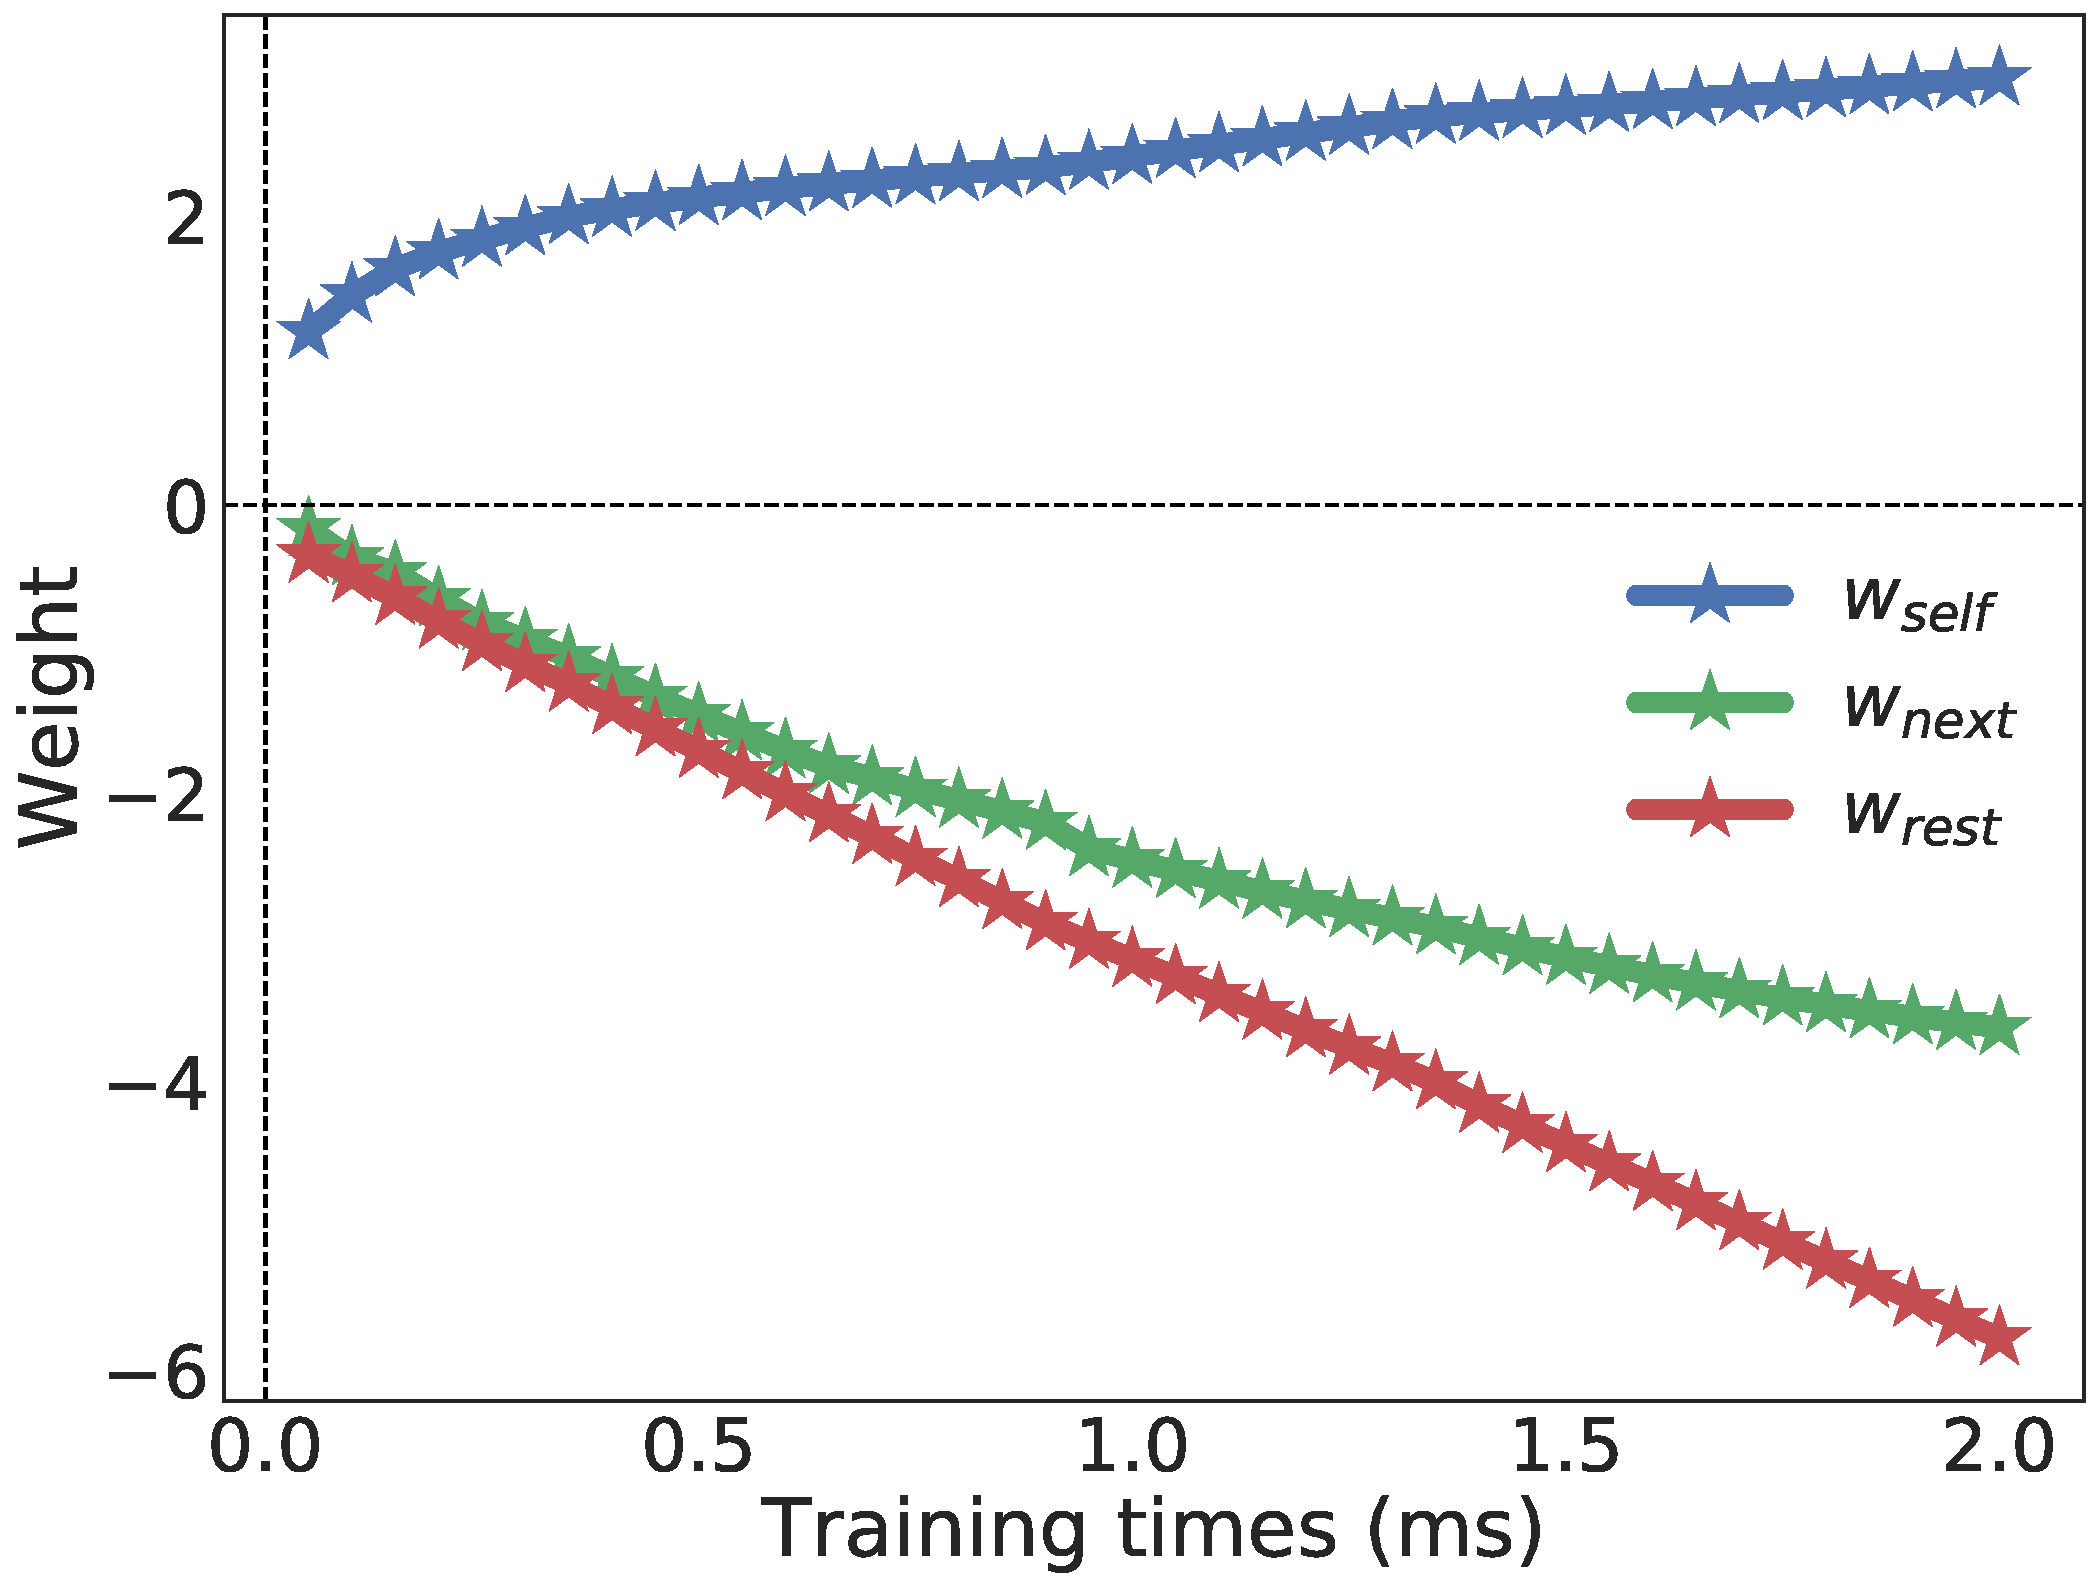
\includegraphics[width=5cm]{simple_bcpnn_training_time.pdf} }}%
    \qquad
    \subfigure[$g_a$]{{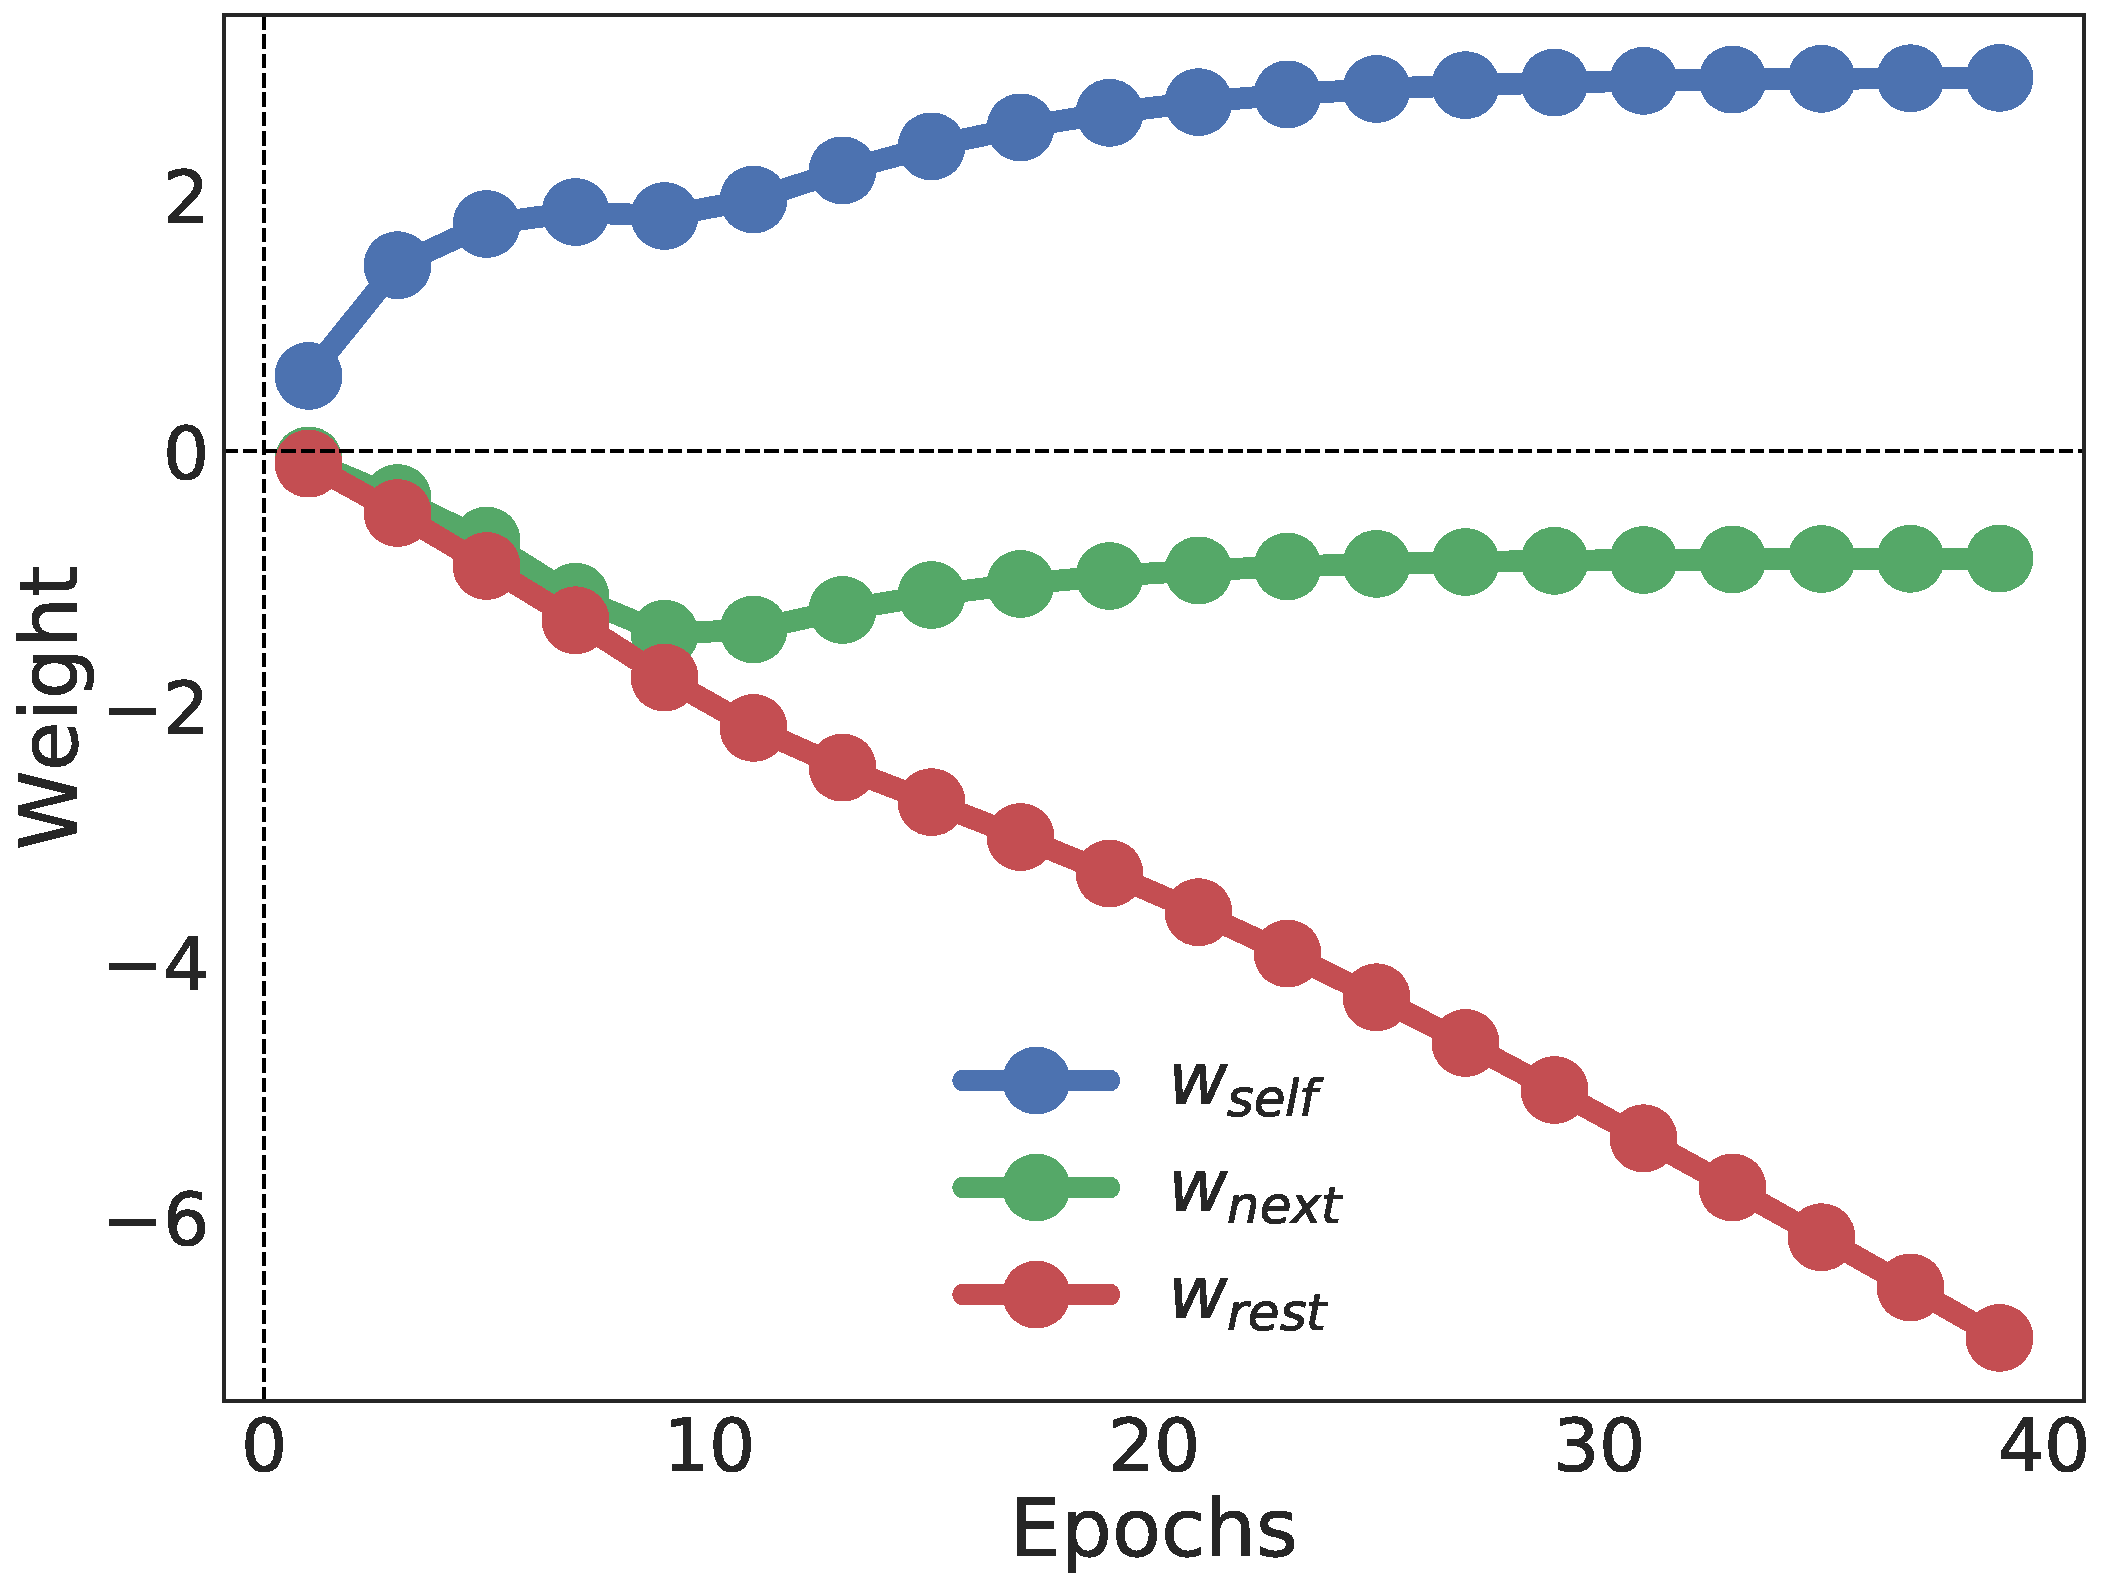
\includegraphics[width=5cm]{simple_bcpnn_epochs.pdf} }}%
    \hfill
    \subfigure[$g_w$]{{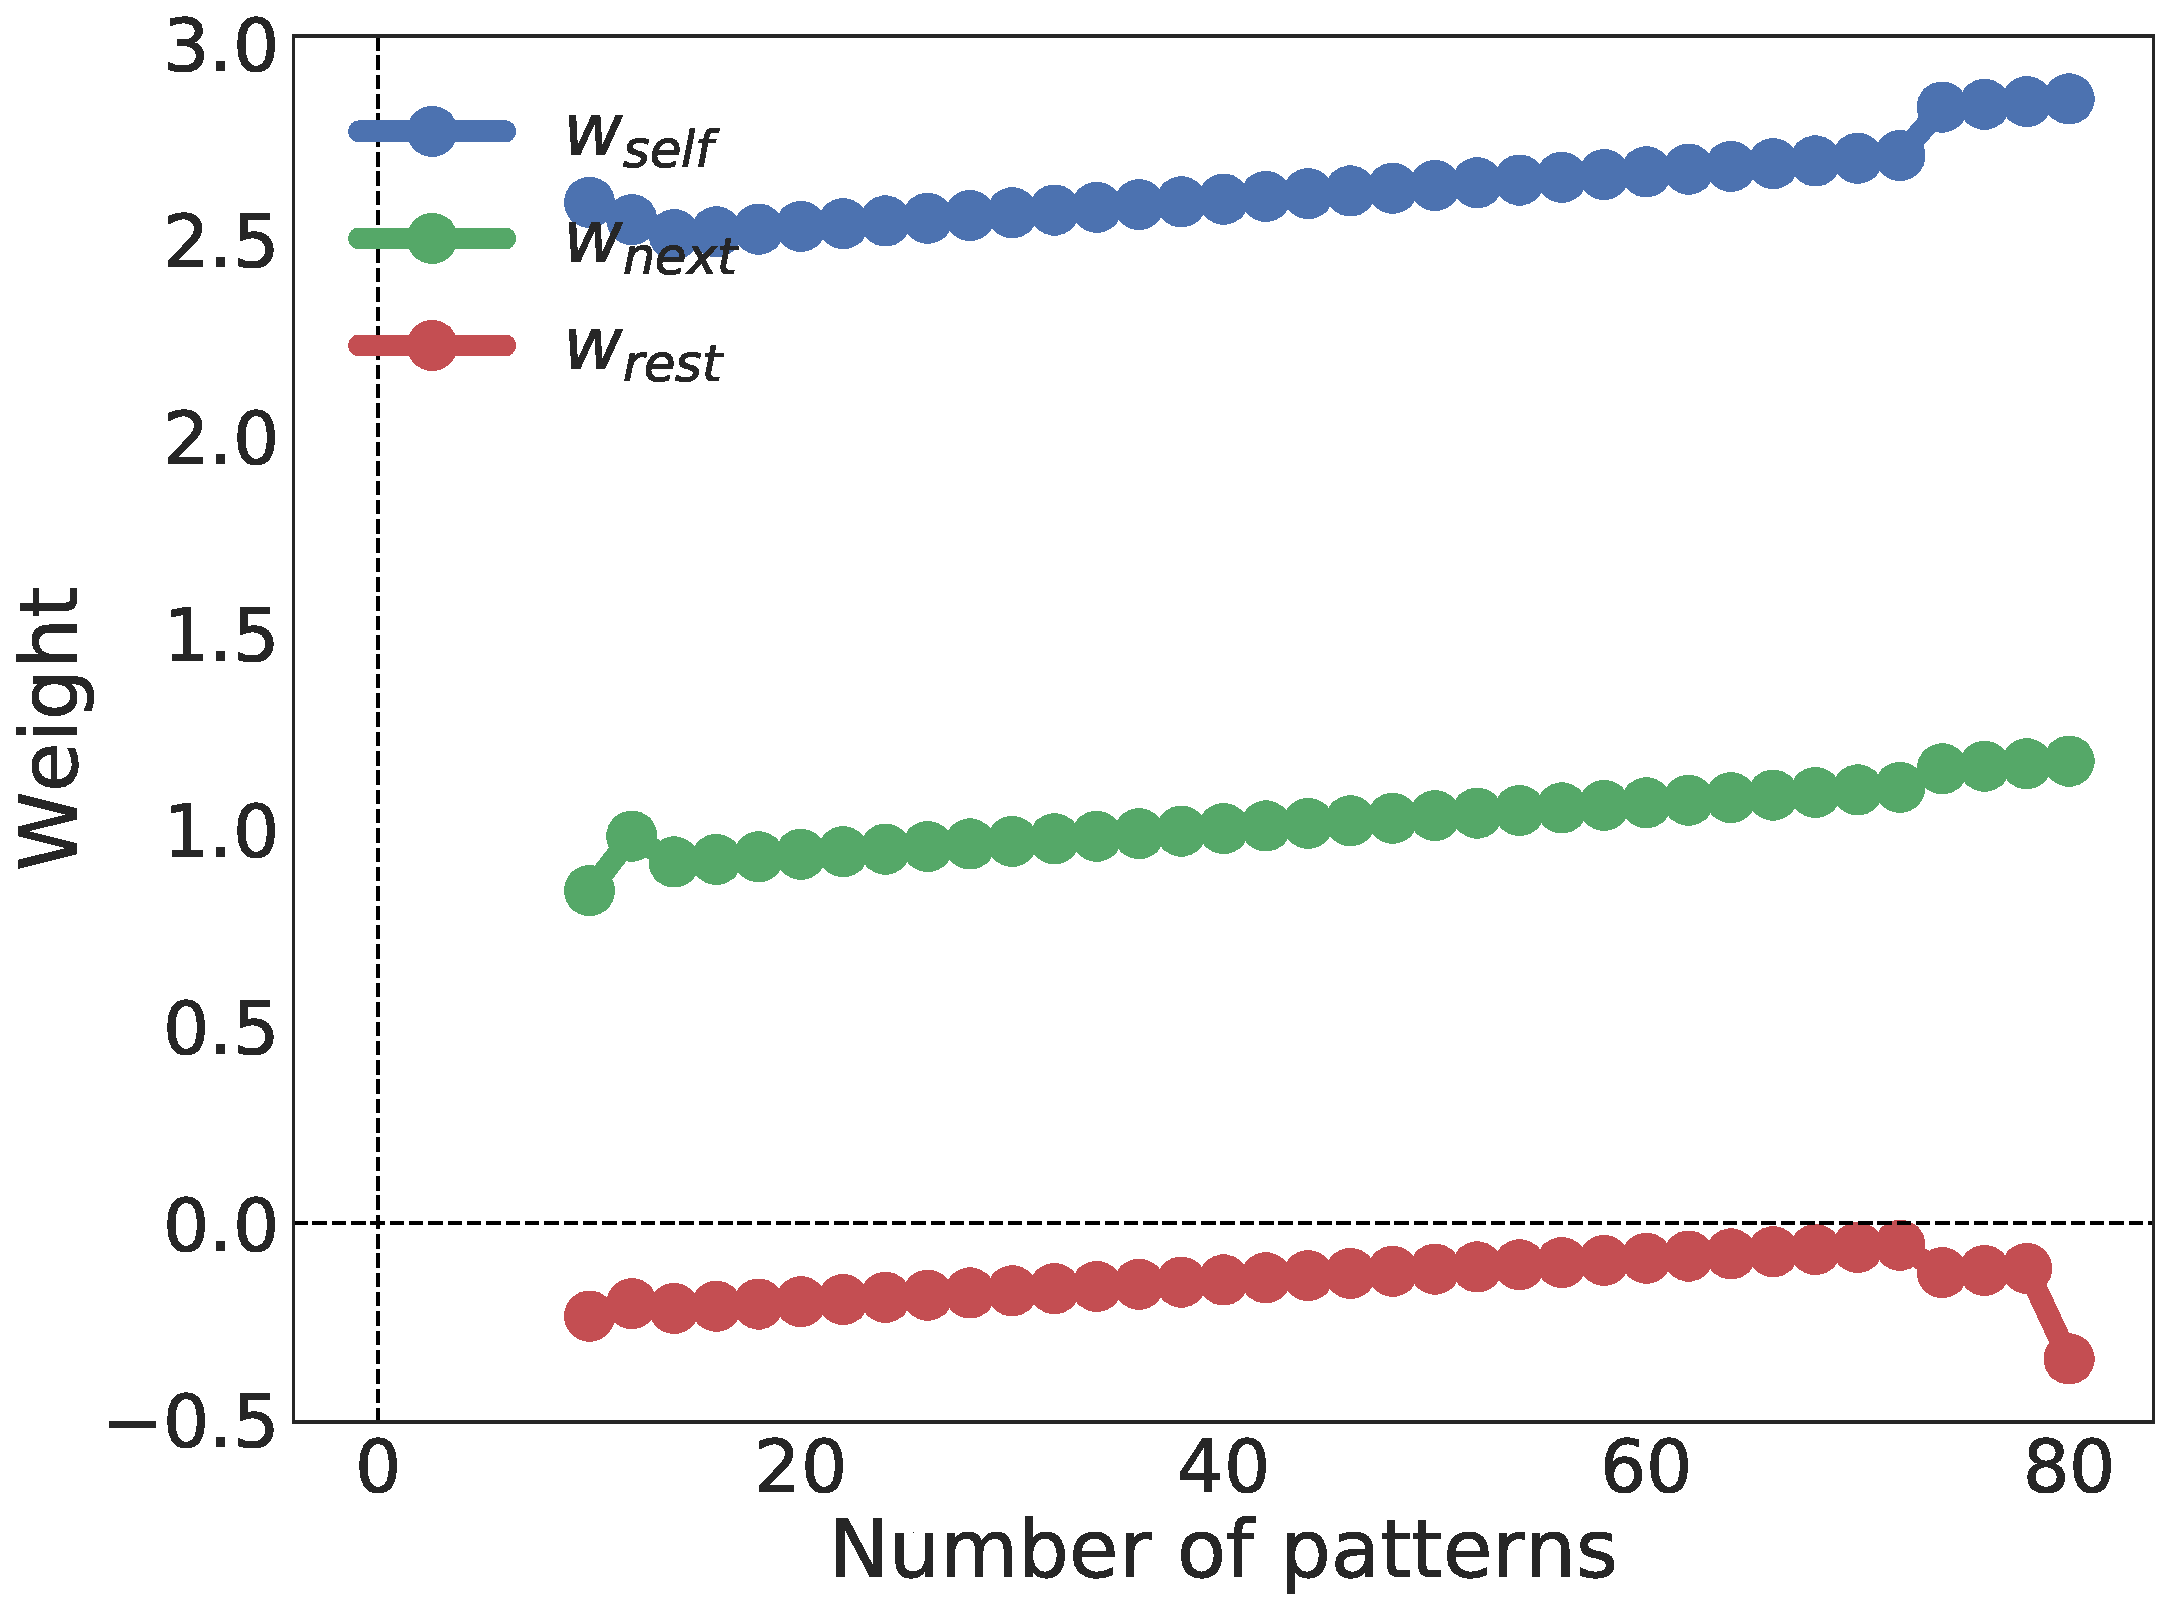
\includegraphics[width=5cm]{simple_bcpnn_patterns.pdf} }}%
     \qquad
    \subfigure[$w_{next}$]{{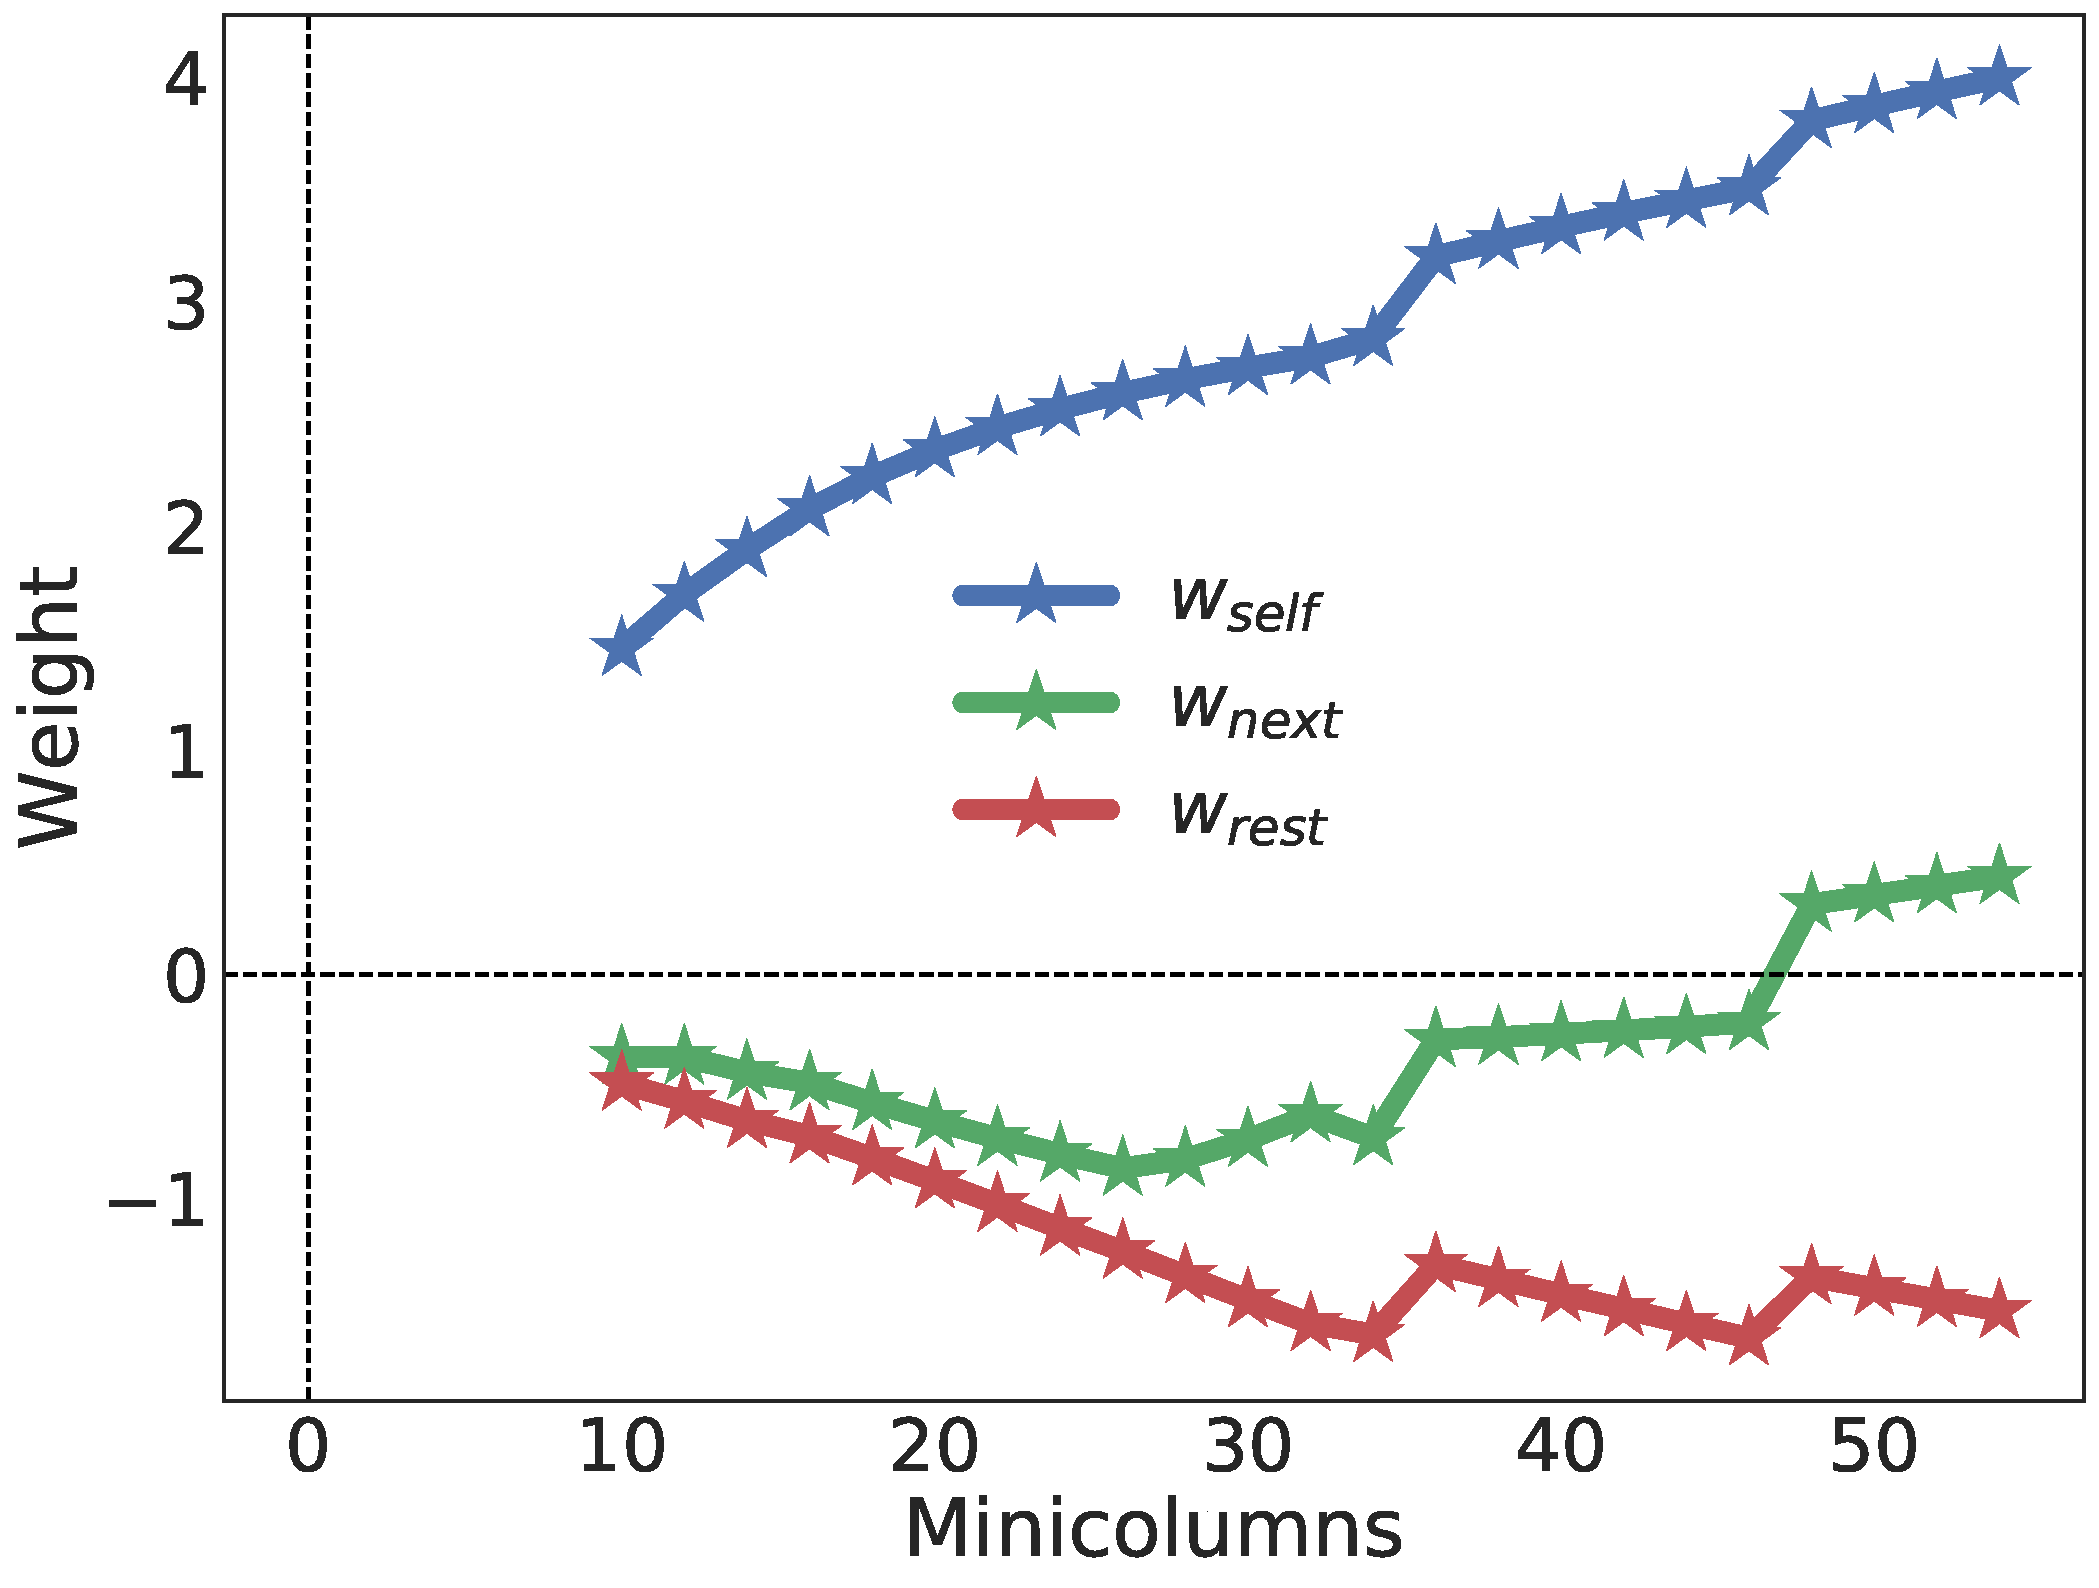
\includegraphics[width=5cm]{simple_bcpnn_minicolumns.pdf} }}%
    \caption{Dynamics of weight learning.   }
    \label{fig:simple_bcpnn_learning}%
\end{figure}


\section{The problem Of Complex Sequences}
Here it is one paper \cite{guyon1988storage}

\bibliographystyle{unsrt}
\bibliography{references.bib}

\end{document}





